\clearpage

\section{Delta Configuration Grammar}

\noindent\begin{minipage}{\textwidth}
  \small
  \begin{align*}
  \langle \textit{Config} \rangle &::= \{ \; \texttt{formulas}: \langle \textit{Formulas} \rangle, \;
      \texttt{variables}: \langle \textit{Vars} \rangle, \;
      \texttt{semantics}: \langle \textit{Sem} \rangle, \\
      &\quad\;\; [\texttt{graph2d}: \langle \textit{G2D} \rangle^*], \;
      [\texttt{graph3d}: \langle \textit{G3D} \rangle^*], \\
      &\quad\;\; [\texttt{stepping}: \textit{bool}], \; \} \\[3pt]
  %
  \langle \textit{Formulas} \rangle &::= [\langle \textit{Formula} \rangle^+] \qquad
  \langle \textit{Formula} \rangle ::= \{ \; \texttt{id}: \textit{str}, \; \texttt{latex}: \textit{str} \; \} \\[3pt]
  %
  \langle \textit{Vars} \rangle &::= \{ \; (\textit{sel} : \textit{num} \mid \langle \textit{VarSpec} \rangle)^* \; \} \\
  \langle \textit{VarSpec} \rangle &::= \{ \; [\texttt{name}: \textit{str}], \;
      [\texttt{default}: \textit{num}], \;
      [\texttt{input}: \texttt{"drag"} \mid \texttt{"inline"}], \\
      &\quad\;\; [\texttt{range}: [\textit{min}, \textit{max}]], \;
      [\texttt{step}], \; [\texttt{precision}], \; [\texttt{sigFigs}], \\
      &\quad\;\; [\texttt{latexDisplay}: \langle \textit{Disp} \rangle], \;
      [\texttt{labelDisplay}: \langle \textit{Disp} \rangle], \\
      &\quad\;\; [\texttt{svgContent}: \langle \textit{SVGFn} \rangle], \;
      [\texttt{svgSize}: \{w,h\}] \; \} \\
  \langle \textit{Disp} \rangle &::= \texttt{"name"} \mid \texttt{"value"} \mid \texttt{"svg"} \mid \texttt{"none"} \\[3pt]
  %
  \langle \textit{Sem} \rangle &::= \texttt{function} \; (\{ \texttt{vars}, \texttt{sample}, \texttt{step}, \texttt{latex} \}) \; \langle \textit{Body} \rangle \\
  \langle \textit{Body} \rangle &::= \{ \; \langle \textit{Stmt} \rangle^* \; \} \\
  \langle \textit{Stmt} \rangle &::= \texttt{vars.}\textit{id} \; \texttt{=} \; \langle \textit{Expr} \rangle \;\mid\;
      \texttt{sample}(\textit{id}, \{ \texttt{x}, \texttt{y}, [\texttt{z}] \}) \\
      &\mid \texttt{step}(\langle \textit{StepSpec} \rangle, [\textit{blockId}]) \;\mid\;
      \texttt{latex}(\textit{n}).\texttt{precision}(\textit{d}) \;\mid\; \langle \textit{JSStmt} \rangle \\
  \langle \textit{StepSpec} \rangle &::= \{ \; [\texttt{description}: \textit{str}], \;
      [\texttt{labels}: \{ (\textit{sel}: \textit{val})^* \}] \; \} \\[3pt]
  %
  \langle \textit{G2D} \rangle &::= \{ \; \texttt{id}: \textit{str}, \;
      [\texttt{xAxisLabel}], \; [\texttt{yAxisLabel}], \;
      [\texttt{xRange}], \; [\texttt{yRange}], \\
      &\quad\;\; [\texttt{lines}: \langle \textit{Line2D} \rangle^*], \;
      [\texttt{points}: \langle \textit{Pt2D} \rangle^*], \;
      [\texttt{vectors}: \langle \textit{Vec} \rangle^*] \; \} \\[3pt]
  %
  \langle \textit{Line2D} \rangle &::= \{ \; \texttt{sampleId}: \textit{str}, \;
      \texttt{parameter}: \textit{sel}, \;
      [\texttt{range}], \; [\texttt{samples}], \;
      [\texttt{interaction}: \langle \textit{Drag} \rangle] \; \} \\
  \langle \textit{Pt2D} \rangle &::= \{ \; \texttt{sampleId}: \textit{str}, \;
      [\texttt{interaction}: \langle \textit{Drag} \rangle], \;
      [\texttt{stepId}], \;
      [\texttt{persistence}] \; \} \\
  \langle \textit{Vec} \rangle &::= \{ \; \texttt{startSampleId}: \textit{str}, \;
      \texttt{endSampleId}: \textit{str}, \;
      [\texttt{label}], \\
      &\quad\;\; [\texttt{interaction}: [\textit{xVar}, \textit{yVar}]], \;
      [\texttt{curved}], \;
      [\texttt{stepId}], \;
      [\texttt{persistence}] \; \} \\
  \langle \textit{Drag} \rangle &::= [\texttt{"horizontal-drag"} \mid \texttt{"vertical-drag"}, \textit{varId}] \\[3pt]
  %
  \langle \textit{G3D} \rangle &::= \{ \; \texttt{id}: \textit{str}, \;
      [\texttt{xRange}], \; [\texttt{yRange}], \; [\texttt{zRange}], \\
      &\quad\;\; [\texttt{surfaces}: \langle \textit{Surf3D} \rangle^*], \;
      [\texttt{lines}: \langle \textit{Line3D} \rangle^*], \;
      [\texttt{points}: \langle \textit{Pt3D} \rangle^*] \; \} \\
  \langle \textit{Surf3D} \rangle &::= \{ \; \texttt{sampleId}: \textit{str}, \;
      \texttt{parameters}: [\textit{v}_1, \textit{v}_2], \;
      [\texttt{ranges}], \; [\texttt{samples}], \; \} \\
  \langle \textit{Line3D} \rangle &::= \{ \; \texttt{sampleId}: \textit{str}, \;
      \texttt{parameter}: \textit{sel}, \;
      [\texttt{range}], \; [\texttt{samples}] \; \} \\
  \langle \textit{Pt3D} \rangle &::= \{ \; \texttt{sampleId}: \textit{str}, \; \}
  \end{align*}
  \captionof{figure}{\textbf{Grammar for Delta configuration language.} \textmd{Styling properties (e.g., \texttt{color}, \texttt{fontSize}, \texttt{labelFontSize}, \texttt{lineWidth}, \texttt{opacity}) and the React component library are omitted. A \textit{sel} (selector) is a LaTeX token (e.g., \texttt{"v"}, \texttt{"\textbackslash\textbackslash mu"}) identifying a variable. Abbreviations: \textit{str}=string, \textit{num}=number, \textit{bool}=boolean. $\langle \textit{Expr} \rangle$ and $\langle \textit{JSStmt} \rangle$ are JavaScript expressions/statements. $\langle \textit{SVGFn} \rangle$ receives the current variable's value and all other variables (\texttt{environment}) from the runtime, returning an SVG string for dynamic variable icons. Square brackets denote optional fields.}}
  \label{fig:bnf-grammar}
  \end{minipage}

\clearpage

\section{Patterns in code from formative analysis}

\begin{minipage}{\textwidth}
\centering
\begin{tabular}{@{}llccccc@{}}
\toprule
\textbf{Article} & \textbf{Source} & \textbf{F1} & \textbf{F2} & \textbf{F3} & \textbf{F4} & \textbf{F5} \\
\midrule
Backprop Explainer            & Individual developer    & $\bullet$ & $\bullet$ & $\bullet$ & $\bullet$ & $\bullet$ \\
Traveling Wave -- Sine Waves  & FigureOne               & $\bullet$ & $\circ$   & $\bullet$ & $\bullet$ & $\bullet$ \\
OLS Regression                & Setosa.io               & $\bullet$ & $\bullet$ & $\bullet$ & $\bullet$ & $\bullet$ \\
Eigenvectors \& Eigenvalues   & Setosa.io               & $\bullet$ & $\bullet$ & $\bullet$ & $\bullet$ & $\bullet$ \\
Why Momentum Really Works     & Distill.pub             & $\bullet$ & $\bullet$ & $\bullet$ & $\bullet$ & $\bullet$ \\
Understanding GNNs            & Distill.pub             & $\bullet$ & $\bullet$ & $\bullet$ & $\bullet$ & $\bullet$ \\
ILA: Least Squares            & Georgia Tech            & $\bullet$ & $\bullet$ & $\bullet$ & $\bullet$ & $\bullet$ \\
ILA: Systems of Equations     & Georgia Tech            & $\bullet$ & $\bullet$ & $\bullet$ & $\bullet$ & $\bullet$ \\
ILA: Vectors                  & Georgia Tech            & $\bullet$ & $\bullet$ & $\bullet$ & $\bullet$ & $\bullet$ \\
Roots of Complex Numbers      & complex-analysis.com    & $\bullet$ & $\circ$   & $\circ$   & $\circ$   & $\bullet$ \\
The Complex Power Function    & complex-analysis.com    & $\bullet$ & $\bullet$ & $\bullet$ & $\bullet$ & $\bullet$ \\
\midrule
\textbf{Total}                &                         & \textbf{11/11} & \textbf{9/11} & \textbf{10/11} & \textbf{10/11} & \textbf{11/11} \\
\bottomrule
\end{tabular}
\captionof{table}{Formative study thematic coding results. \textmd{Each cell indicates whether the pattern was observed ($\bullet$) or not ($\circ$) in the article's source repository. Codes for frictions: \textbf{F1}~Diffuseness and tangling, \textbf{F2}~Indirect identifiers, \textbf{F3}~Fussing the DOM and LaTeX, \textbf{F4}~Repetition, \textbf{F5}~State management. See Section~\ref{FormativeStudy} for definitions.}}
\label{tab:formative-audit}
\end{minipage}

\clearpage

\section{Examples from formative analysis}

\begin{minipage}{\textwidth}
\centering
\begin{minipage}[t]{0.48\textwidth}
\begin{lstlisting}[basicstyle=\ttfamily\scriptsize, frame=single, title={\texttt{fig2.js:123--139} (amplitude control)}]
let offset = 0.5;
mover.notifications.add('setTransform', () => {
  offset += mover.getPosition().y * 2;
  mover.transform.updateTranslation([0, 0]);
  if (offset > 1) { offset = 1; }
  if (offset < -1) { offset = -1; }
  const newA = offset * 2;
  trace.update(sine(newA));
  eqn.updateElementText({
    A: `${Math.abs(newA).toFixed(1)}`,
    sign
  });
});
\end{lstlisting}
\end{minipage}
\hfill
\begin{minipage}[t]{0.48\textwidth}
\begin{lstlisting}[basicstyle=\ttfamily\scriptsize, frame=single, title={\texttt{fig3.js:129--142} (wavelength control)}]
let offset = 0;
mover.notifications.add('setTransform', () => {
  offset += mover.getPosition().x;
  mover.transform.updateTranslation([0, 0.15]);
  if (offset > 1) { offset = 1; }
  if (offset < -1) { offset = -1; }
  const newR = offset * 3 + 5;
  trace.update(sine(newR));
  eqn.updateElementText({
    value: `${newR.toFixed(1)}`
  });
});
\end{lstlisting}
\end{minipage}
\captionof{figure}{\textbf{Schema duplication in the Traveling Wave article~\cite{FigureOne-TravelingWave}.} \textmd{Two figures implement the same interaction schema---a draggable parameter controlling a sine wave---with structurally identical code. Both blocks maintain local \texttt{offset} state, accumulate drag input, clamp to bounds, transform to a parameter value, update the trace, and refresh the equation label. The only differences are which axis is read (\texttt{.y} vs \texttt{.x}), which parameter is computed (\texttt{newA} vs \texttt{newR}), and which label field is updated. This pattern, where the same mathematical interaction schema is copy-pasted and lightly edited per instance, appeared in 10 of 11 audited articles.}}
\label{fig:schema-duplication}
\end{minipage}

\begin{minipage}{\textwidth}
\centering
\begin{minipage}[t]{0.48\textwidth}
\begin{lstlisting}[basicstyle=\ttfamily\scriptsize, frame=single, title={OLS Regression: DOM geometry for highlight positioning}]
// After render, measure tspan elements
var svgBB = this.getDOMNode().getBoundingClientRect();
var beta1Text = this.refs.beta1Text.getDOMNode();
var beta1TextBB = beta1Text.getClientRects()[0];
var beta2Text = this.refs.beta2Text.getDOMNode();
var beta2TextBB = beta2Text.getClientRects()[0];

// Manually reposition highlight overlays
d3.select(this.refs.beta1Highlight.getDOMNode())
  .attr('transform',
    `translate(${highlight1Pos.x}, ${highlight1Pos.y})`);
d3.select(this.refs.beta2Highlight.getDOMNode())
  .attr('transform',
    `translate(${highlight2Pos.x}, ${highlight2Pos.y})`);
\end{lstlisting}
\end{minipage}
\hfill
\begin{minipage}[t]{0.48\textwidth}
\begin{lstlisting}[basicstyle=\ttfamily\scriptsize, frame=single, title={Why Momentum Really Works: HTML string replacement}]
// Cache rendered MathJax in hidden DOM
function MathCache(id) {
  return document.querySelector(
    "#math-cache ." + id).innerHTML;
}

// String-replace inside rendered formula HTML
function renderEquation(hat, value, number) {
  var html = hat ? MathCache("phat")
                 : MathCache("p");
  html = html.replace(
    '<span class="mord mathrm">0</span>', value);
  html = html.replace(
    '<span class="mord mathrm mtight">1</span>', number);
  return html;
}
\end{lstlisting}
\end{minipage}
\captionof{figure}{\textbf{Fussing the DOM and \LaTeX{} (F3).} \textmd{Left: the OLS Regression article~\cite{setosa-ols} measures rendered \texttt{tspan} bounding boxes after each React render, then manually repositions SVG highlight groups with \texttt{translate()} transforms. Right: the Momentum article~\cite{goh2017why} caches rendered MathJax fragments in a hidden DOM element, retrieves them via \texttt{querySelector}, and performs string replacement on the internal \texttt{<span>} markup to swap in dynamic values. Both patterns require authors to understand renderer internals and coordinate between mathematical intent and low-level DOM structure.}}
\label{fig:latex-dom-manipulation}
\end{minipage}

\clearpage

\begin{minipage}{\textwidth}
\centering
\begin{minipage}[t]{0.48\textwidth}
\begin{lstlisting}[basicstyle=\ttfamily\scriptsize, frame=single, title={Backprop Explainer: deeply nested state object}]
// Bespoke nested state for regression
this.state = {
  yhat: [],
  playButton: true,
  linreg: {
    data: { X: [], y: [] },
    hyperparams: {
      learningRate: 0.03,
      epochs: 0,
      loss: null,
      speed: 200
    },
    tunableparams: { m: 0, b: 0 }
  }
};

// Manual event wiring to state transitions
<Fab onClick={async () => {
  await this.setState({
    playButton: !this.state.playButton });
  await this.a();
}}>
\end{lstlisting}
\end{minipage}
\hfill
\begin{minipage}[t]{0.48\textwidth}
\begin{lstlisting}[basicstyle=\ttfamily\scriptsize, frame=single, title={Eigenvectors: manual derived-value propagation}]
// Mutable state object
var opt = $scope.opt = {};
opt.pos0 = [2, 3];
opt.basis1 = [1, 0.5];
opt.basis2 = [0.5, 1];
opt.eigenVectors = [[1, 0], [0, 1]];
opt.eigenValues = [0, 0];

// Deep watch triggers manual recomputation
$scope.$watch('opt', function() {
  derived($scope)
}, true);

// Low-level drag wiring
nobs.call(d3.behavior.drag()
  .on('drag', function(d) {
    scope.$apply(function() {
      d.set(scope, d3.mouse(svg.node()))
    })
  }));
\end{lstlisting}
\end{minipage}
\captionof{figure}{\textbf{State management (F5).} \textmd{Left: the Backprop Explainer~\cite{backprop-explainer} maintains a deeply nested state object mixing UI flags (\texttt{playButton}), data arrays, hyperparameters, and tunable parameters, then wires click handlers to async state transitions. Right: the Eigenvectors article~\cite{setosa-eigen} stores mutable state in an Angular scope object, uses a deep \texttt{\$watch} to trigger manual recomputation of derived quantities, and wires D3 drag events through framework-specific \texttt{\$apply} calls. Both patterns require authors to manually orchestrate state flow, derived-value updates, and framework integration.}}
\label{fig:custom-state}
\end{minipage}
% \end{figure*}

\clearpage

% \subsection{Delta Language Grammar}

% \begin{table}[h]
% \small
% \centering
% \begin{tabular}{@{}p{0.46\columnwidth}p{0.46\columnwidth}@{}}
% \toprule
% \textbf{Traditional MathJax} & \textbf{Delta} \\
% \midrule
% Configure \texttt{window.MathJax} & Automatic \\
% Inject \texttt{<script>} tag & Dynamic injection \\
% Await startup promise & Gated rendering \\
% Call \texttt{tex2chtml()} & Handled by \texttt{Formula} \\
% Manual re-typesetting & Reactive via MobX \\
% \bottomrule
% \end{tabular}
% \caption{MathJax setup responsibilities absorbed by Delta.}
% \label{tab:mathjax-comparison}
% \end{table}

% \begin{table}[h]
% \small
% \centering
% \caption{Variable properties in Delta.}
% \label{tab:variable-properties}
% \begin{tabularx}{\columnwidth}{@{}lXX@{}}
% \toprule
% Property & Purpose & Example \\
% \midrule
% \texttt{input} & Interaction type & \texttt{"drag"}, \texttt{"inline"} \\
% \texttt{default} & Starting value & \texttt{0.5} \\
% \texttt{range} & Min/max bounds & \texttt{[-1, 4]} \\
% \texttt{step} & Drag increment & \texttt{0.05} \\
% \texttt{name} & Display label & \texttt{"Learning Rate"} \\
% \texttt{precision} & Decimal places & \texttt{2} \\
% \texttt{sigFigs} & Significant figures & \texttt{4} \\
% \texttt{latexDisplay} & Name or value in formula & \texttt{"name"}, \texttt{"value"}, \texttt{"svg"} \\
% \texttt{labelDisplay} & Label rendering mode & \texttt{"name"}, \texttt{"value"}, \texttt{"svg"}, \texttt{"none"} \\
% \bottomrule
% \end{tabularx}
% \end{table}

% \begin{table}[h]
% \footnotesize
% \centering
% \caption{Semantics context: \texttt{vars} proxy and helper functions.}
% \label{tab:vars-access}
% \begin{tabular}{@{}p{0.28\columnwidth}p{0.22\columnwidth}p{0.42\columnwidth}@{}}
% \toprule
% Syntax & Use case & Example \\
% \midrule
% \texttt{vars.x} & Simple symbols & \texttt{vars.K = 0.5 * vars.m} \\
% \texttt{vars["..."]} & LaTeX tokens & \texttt{vars["\textbackslash\textbackslash mu"] = sum / n} \\
% \texttt{sample(id, \{x, y\})} & Emit data point & \texttt{sample("curve", \{x: t, y: f\})} \\
% \texttt{latex(n).precision(d)} & Format number & \texttt{latex(3.14).precision(2)} \\
% \bottomrule
% \end{tabular}
% \end{table}

% \begin{table}[h]
% \small
% \centering
% \caption{\texttt{Custom()} component API for building reactive visualizations.}
% \label{tab:custom-api}
% \begin{tabularx}{\columnwidth}{@{}lX@{}}
% \toprule
% Feature & Description \\
% \midrule
% \texttt{Custom(render)} & Wraps a render function to create a reactive component \\
% \texttt{vars.x} (read) & Returns current value of variable \texttt{x} \\
% \texttt{vars.x = v} (write) & Updates variable \texttt{x}, triggering re-computation \\
% Auto re-render & Component re-renders when any accessed variable changes \\
% \bottomrule
% \end{tabularx}
% \end{table}

\section{Example Delta specs}

\begin{minipage}{\textwidth}
\centering
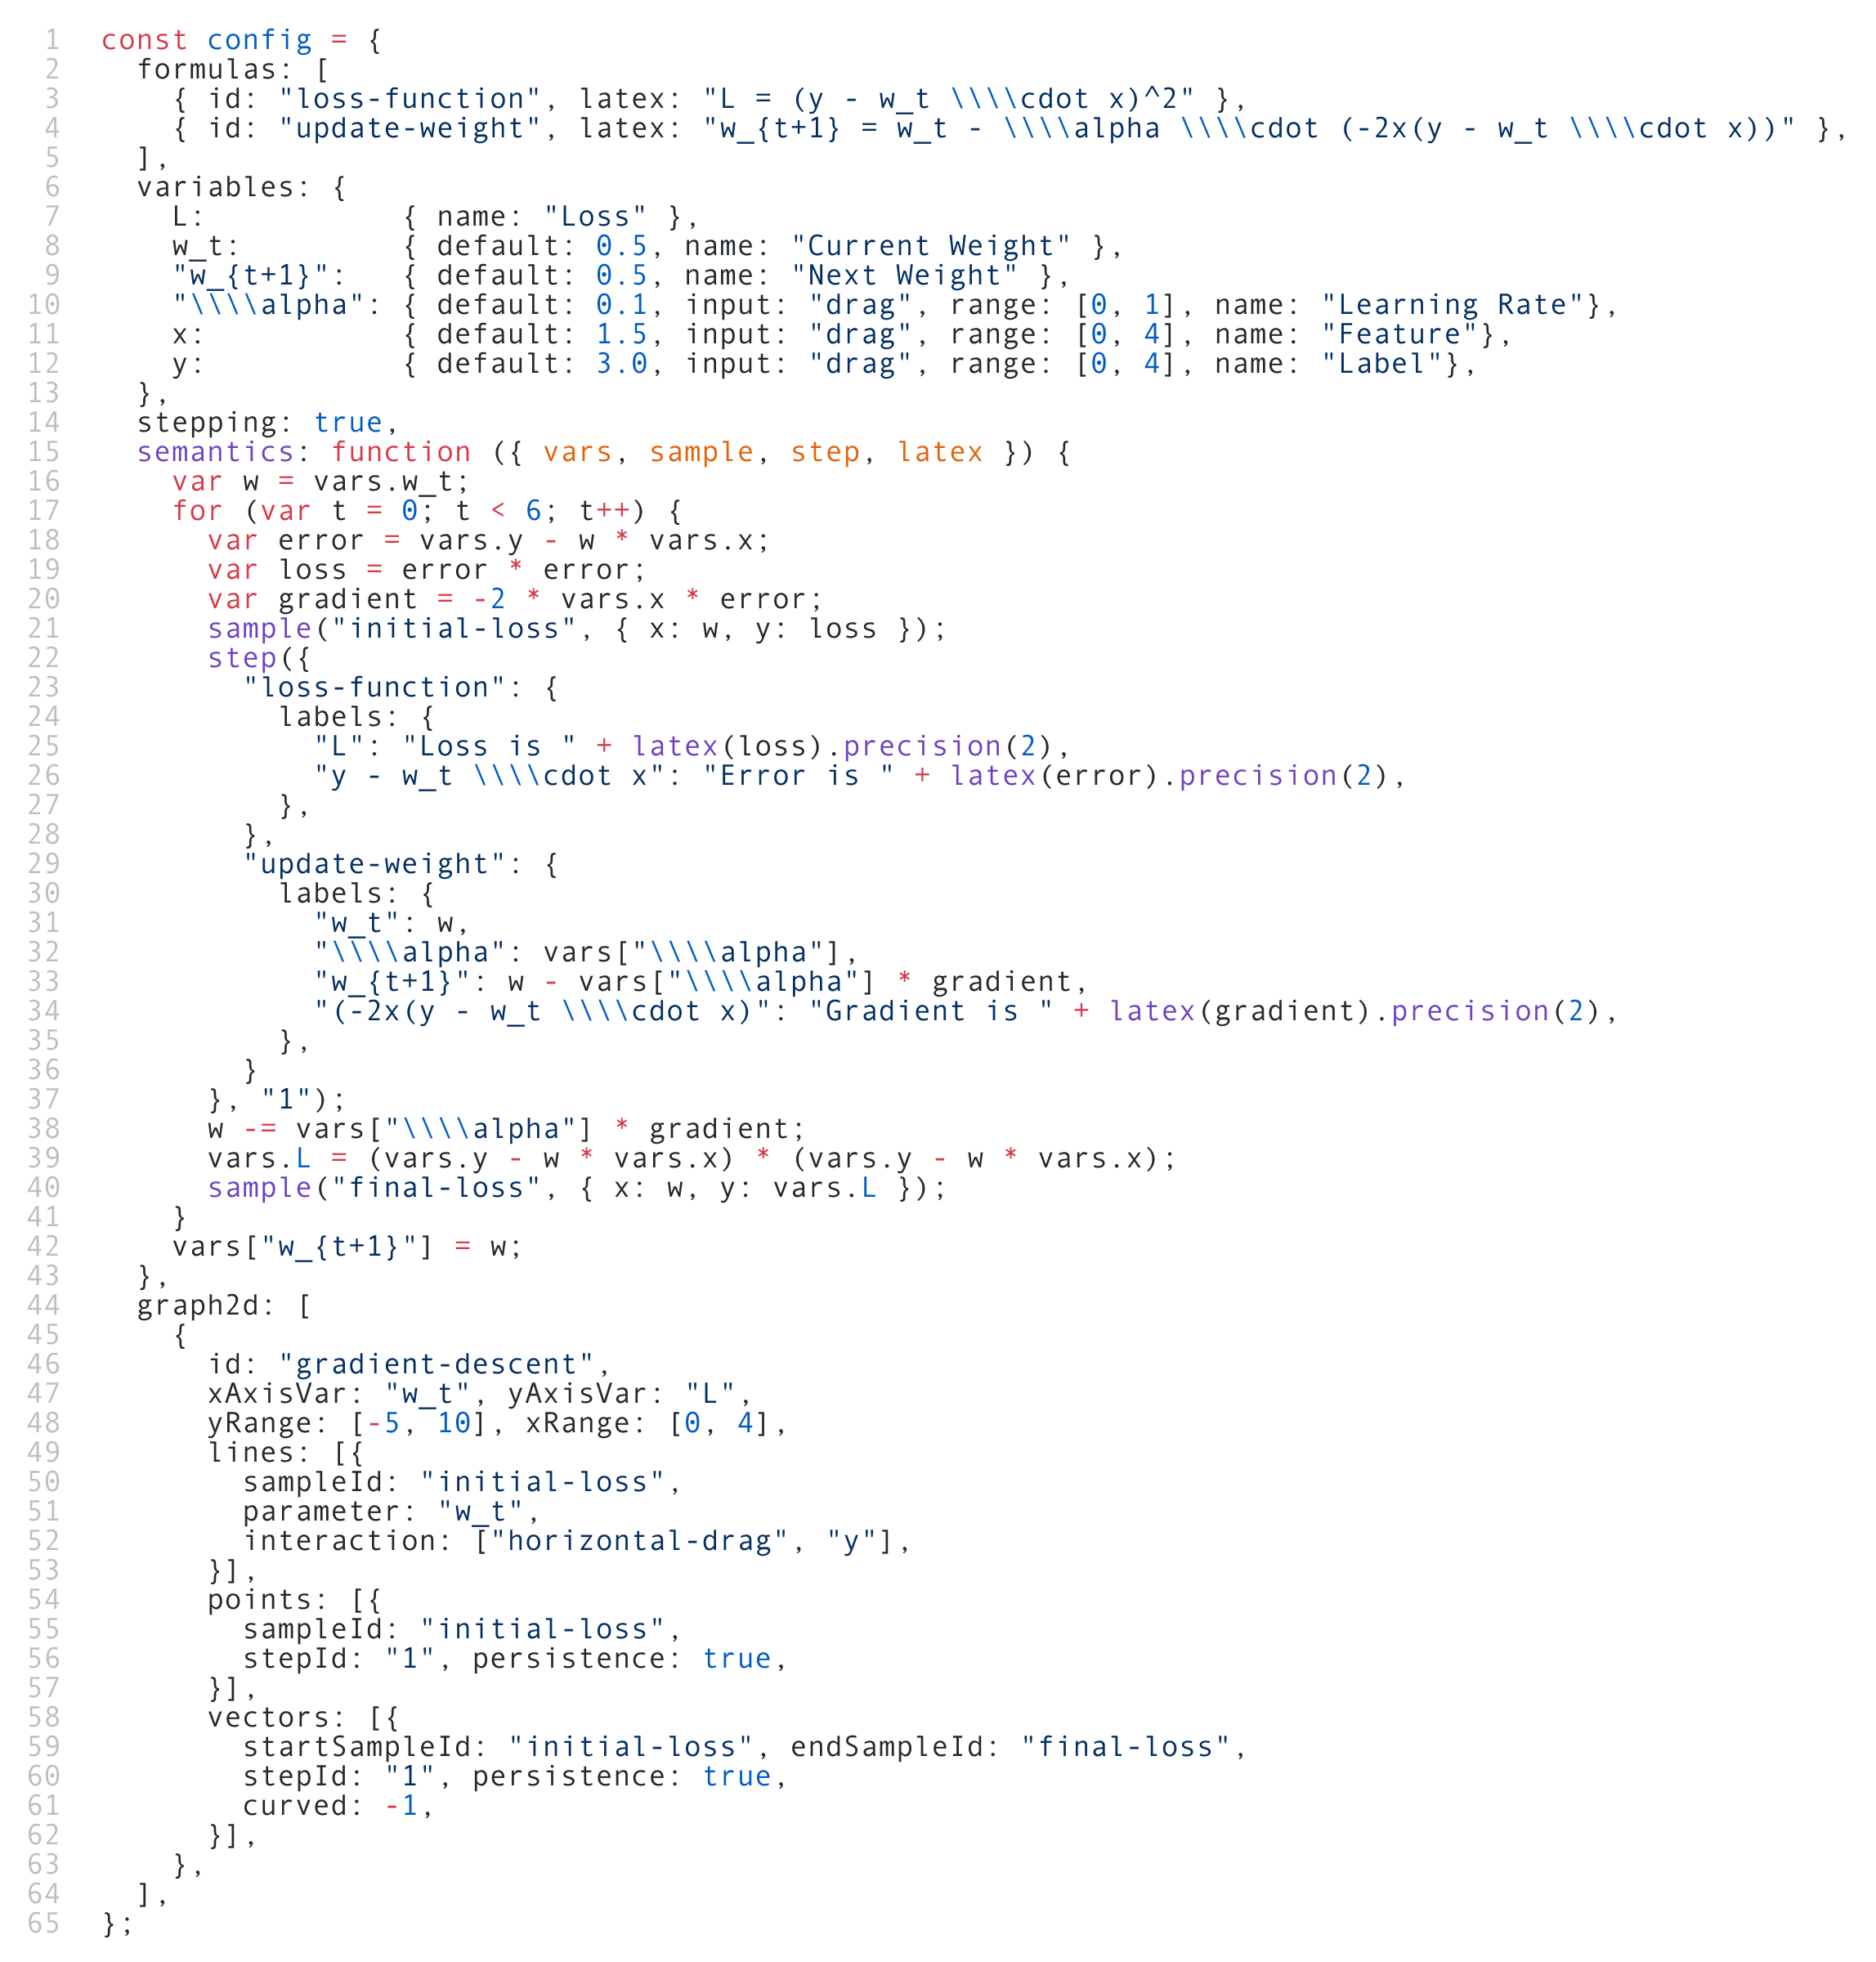
\includegraphics[width=\textwidth]{fig/gradient.png}
\captionof{figure}{Delta configuration for gradient descent walkthrough (Figure~\ref{fig:system}). \textmd{The specification declares two formulas, five interactive variables, and a semantics function that loops through training iterations, emitting \texttt{step()} calls with labels keyed by formula \texttt{id}.}}
\label{fig:gradient-config}
\end{minipage}

\clearpage

\section{Study 1 Details}

\subsubsection{Participant backgrounds}

Participants rated their comfort writing LaTeX formulas as a median of 4 on a 5-point Likert scale ($\sigma = 0.91$); 11 wrote LaTeX weekly, 5 monthly, and 3 less than monthly. They rated their comfort writing JavaScript as a median of 4 ($\sigma = 1.12$); 9 wrote JS weekly, 8 monthly, 1 daily, and 1 less than monthly. Regarding React experience, 6 had written substantial amounts of React in a professional context, 6 had written substantial amounts in personal or academic projects, and 7 had written small amounts in personal or academic projects. We refer to these participants by anonymized random double-digit numeric identifiers (e.g., P21, P48).

\subsubsection{Task time by order of interface assignment}
\label{sec:order-effect}

We observed a significant order effect on the magnitude of the time difference between conditions (Mann-Whitney $U = 88.0$, $p < .001$). Participants who used the baseline first showed a larger advantage for Delta (mean difference $= 8.9$ min) than those who used Delta first (mean difference $= 1.8$ min). This suggests that task familiarity compressed completion times in the second condition regardless of library. Critically, even within the more conservative subgroup that used Delta \textit{first}, Delta was still significantly faster (Wilcoxon $W = 6.0$, $p = .027$, $n = 10$), with 7 of 10 participants completing the task faster with Delta.

\subsubsection{Analysis of participant free-text responses}
\label{sec:free-text-analysis}

Participants' free-text responses revealed qualitative differences in \textit{where} each tool imposed cognitive load. We organize these findings using the Cognitive Dimensions of Notations framework~\cite{Blackwell2003-gv}, a widely adopted vocabulary for evaluating the usability of programming languages and notation systems. Three dimensions emerged most clearly.

\paragraph{Viscosity.} 
The most frequently cited baseline pain point was the effort required to make even a small change. Seven participants (P45, P55, P79, P80, P87, P88, P99) described the baseline as requiring coordinated edits across disconnected locations---state declarations, component props, and the LaTeX string (P55: ``making the small change to make m modifiable with a drag motion required changes in several parts of the code''). The \texttt{\textbackslash cssId\{\}} mechanism was a specific source of friction: seven participants (P11, P14, P20, P79, P87, P88, P99) reported confusion or errors matching CSS identifiers across component props and LaTeX strings (e.g., P88: ``I forgot to add the cssId on the LaTeX element `m'\,'').

\paragraph{Closeness of mapping.}
Four participants (P11, P20, P79, P88) independently described Delta's structure---formulas, variables, and semantics---in terms that closely mirror the library's API, without being prompted. P11 explained: ``there's the semantics of a formula, the looks of a formula [LaTeX], and then different components of the formula. [Delta] naturally gave in to this description.'' [Delta] had these components and only these that I need to change.'' That participants independently reconstructed the library's decomposition suggests it maps closely to how authors naturally reason about interactive formula authoring.

\paragraph{Visibility.}
Delta's configuration also improved \emph{visibility}---the ease with which required parts of the notation can be identified. Ten of 19 participants cited co-location as an advantage: P29 found it ``way faster to just look at the code and immediately see all the moving parts at a glance''; P21 praised ``clear partitions for variables, so could find and update easily''; and P80 described Delta as grouping ``the variables/components (labels, dragging functionality, displayed value) together in an intuitive way.'' By contrast, the baseline scattered relevant parts across disconnected locations (P79: ``a lot of moving components---in the html, use state, two types of wrappers'').

Two participants (P29, P14) preferred the baseline on suitability and language dimensions despite completing the task faster with Delta, citing familiarity with React idioms---pointing to a tension between task-specific efficiency and integration with existing workflows.

\clearpage

\section{Study 2 details}

\begin{minipage}{\columnwidth}
\centering
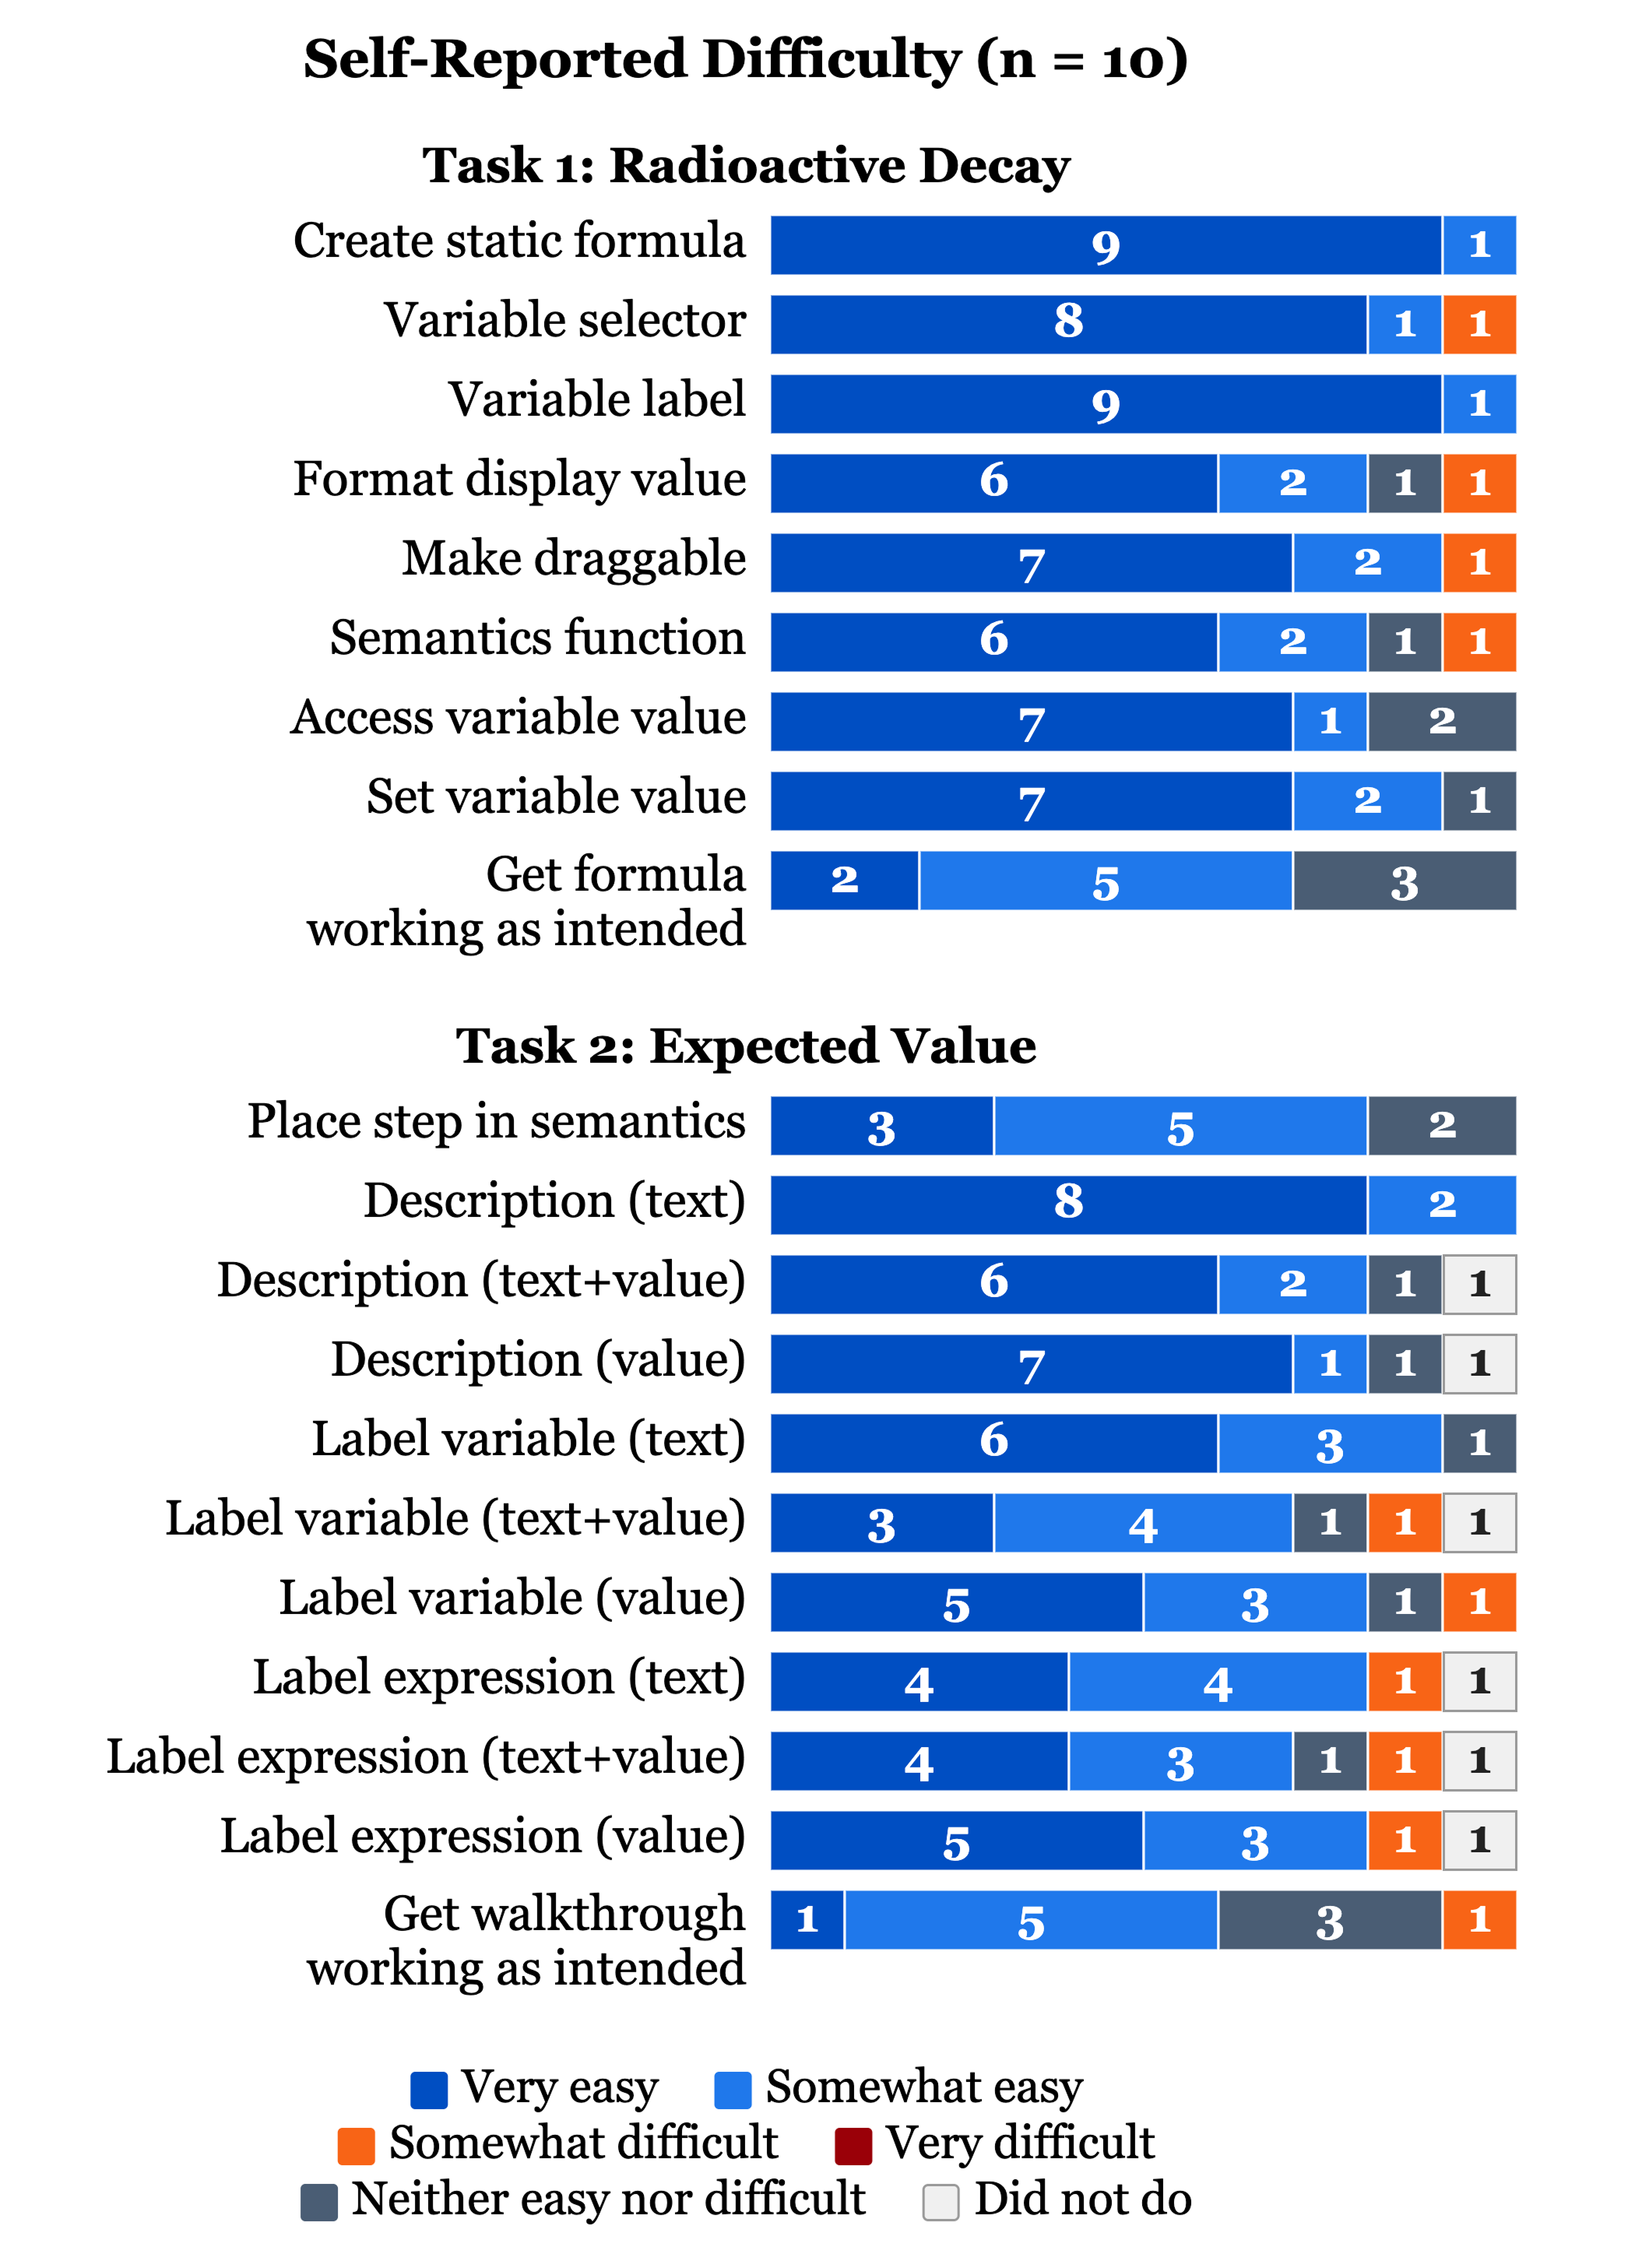
\includegraphics[width=\linewidth]{fig/difficulty.png}
\captionof{figure}{\textbf{Self-reported difficulty ratings.} Authors rated the difficulty of library features on a 5-point Likert scale ($n = 10$; some Task~2 features $n = 9$ due to ``did not do'' responses). \textmd{The distribution largely mirrors the intuitiveness ratings (Figure~\ref{fig:obs-intuitiveness}), with most features rated as easy or very easy.}}
\Description{Diverging stacked bar chart showing Likert-scale difficulty responses for both tasks side by side. The distribution is similar to the intuitiveness ratings, with most bars dominated by blue (very easy / somewhat easy).}
\label{fig:obs-difficulty}
\end{minipage}